% ============================================================
% 用户手册 — 时序数据采集与应用管理系统
% 操作指南：每个模块怎么用
% ============================================================
\documentclass[11pt,a4paper]{ctexart}
\usepackage{xeCJK,xcolor,graphicx,float,fancyhdr,hyperref,geometry,booktabs,enumitem}
\setCJKmainfont{Microsoft YaHei}
\geometry{a4paper,margin=2.2cm}
\pagestyle{fancy}
\fancyhead[L]{时序数据采集与应用管理系统 — 用户手册}
\fancyhead[R]{V1.0}
\fancyfoot[C]{\thepage}

\begin{document}

\begin{center}
{\Huge\bfseries 时序数据采集与应用管理系统\\[8pt] 用户手册}\\[14pt]
{\large 操作指南：每个模块怎么用}\\[8pt]
{\large 版本 V1.0 \quad 2026-08}
\end{center}
\vspace{1em}\noindent\hrulefill\vspace{1em}

\section{快速入门}

\subsection{系统入口}

系统提供两个入口，面向不同角色：

\begin{itemize}[leftmargin=*]
  \item \textbf{驾驶舱大屏}：面向领导和管理人员，一屏总览全油田运行状态，无需登录操作
  \item \textbf{管理后台}：面向运维和业务人员，9 大功能模块提供全部管理操作
\end{itemize}

\subsection{登录}

打开浏览器访问系统地址，进入登录页面。输入用户名和密码后点击登录，系统将根据用户角色自动加载对应的界面权限。

\subsection{界面布局}

登录后进入管理后台，界面分为三个区域：

\begin{itemize}[leftmargin=*]
  \item \textbf{顶部状态条}：系统运行状态指示灯、全局搜索框、告警铃铛（显示未处置告警数量）、当前登录用户
  \item \textbf{左侧导航栏}：① 驾驶舱 ~ ⑨ 系统管理 共 9 个功能模块入口，点击切换
  \item \textbf{主工作区}：随所选模块切换，显示列表/详情/图表/配置表单
\end{itemize}

\begin{figure}[H]\centering
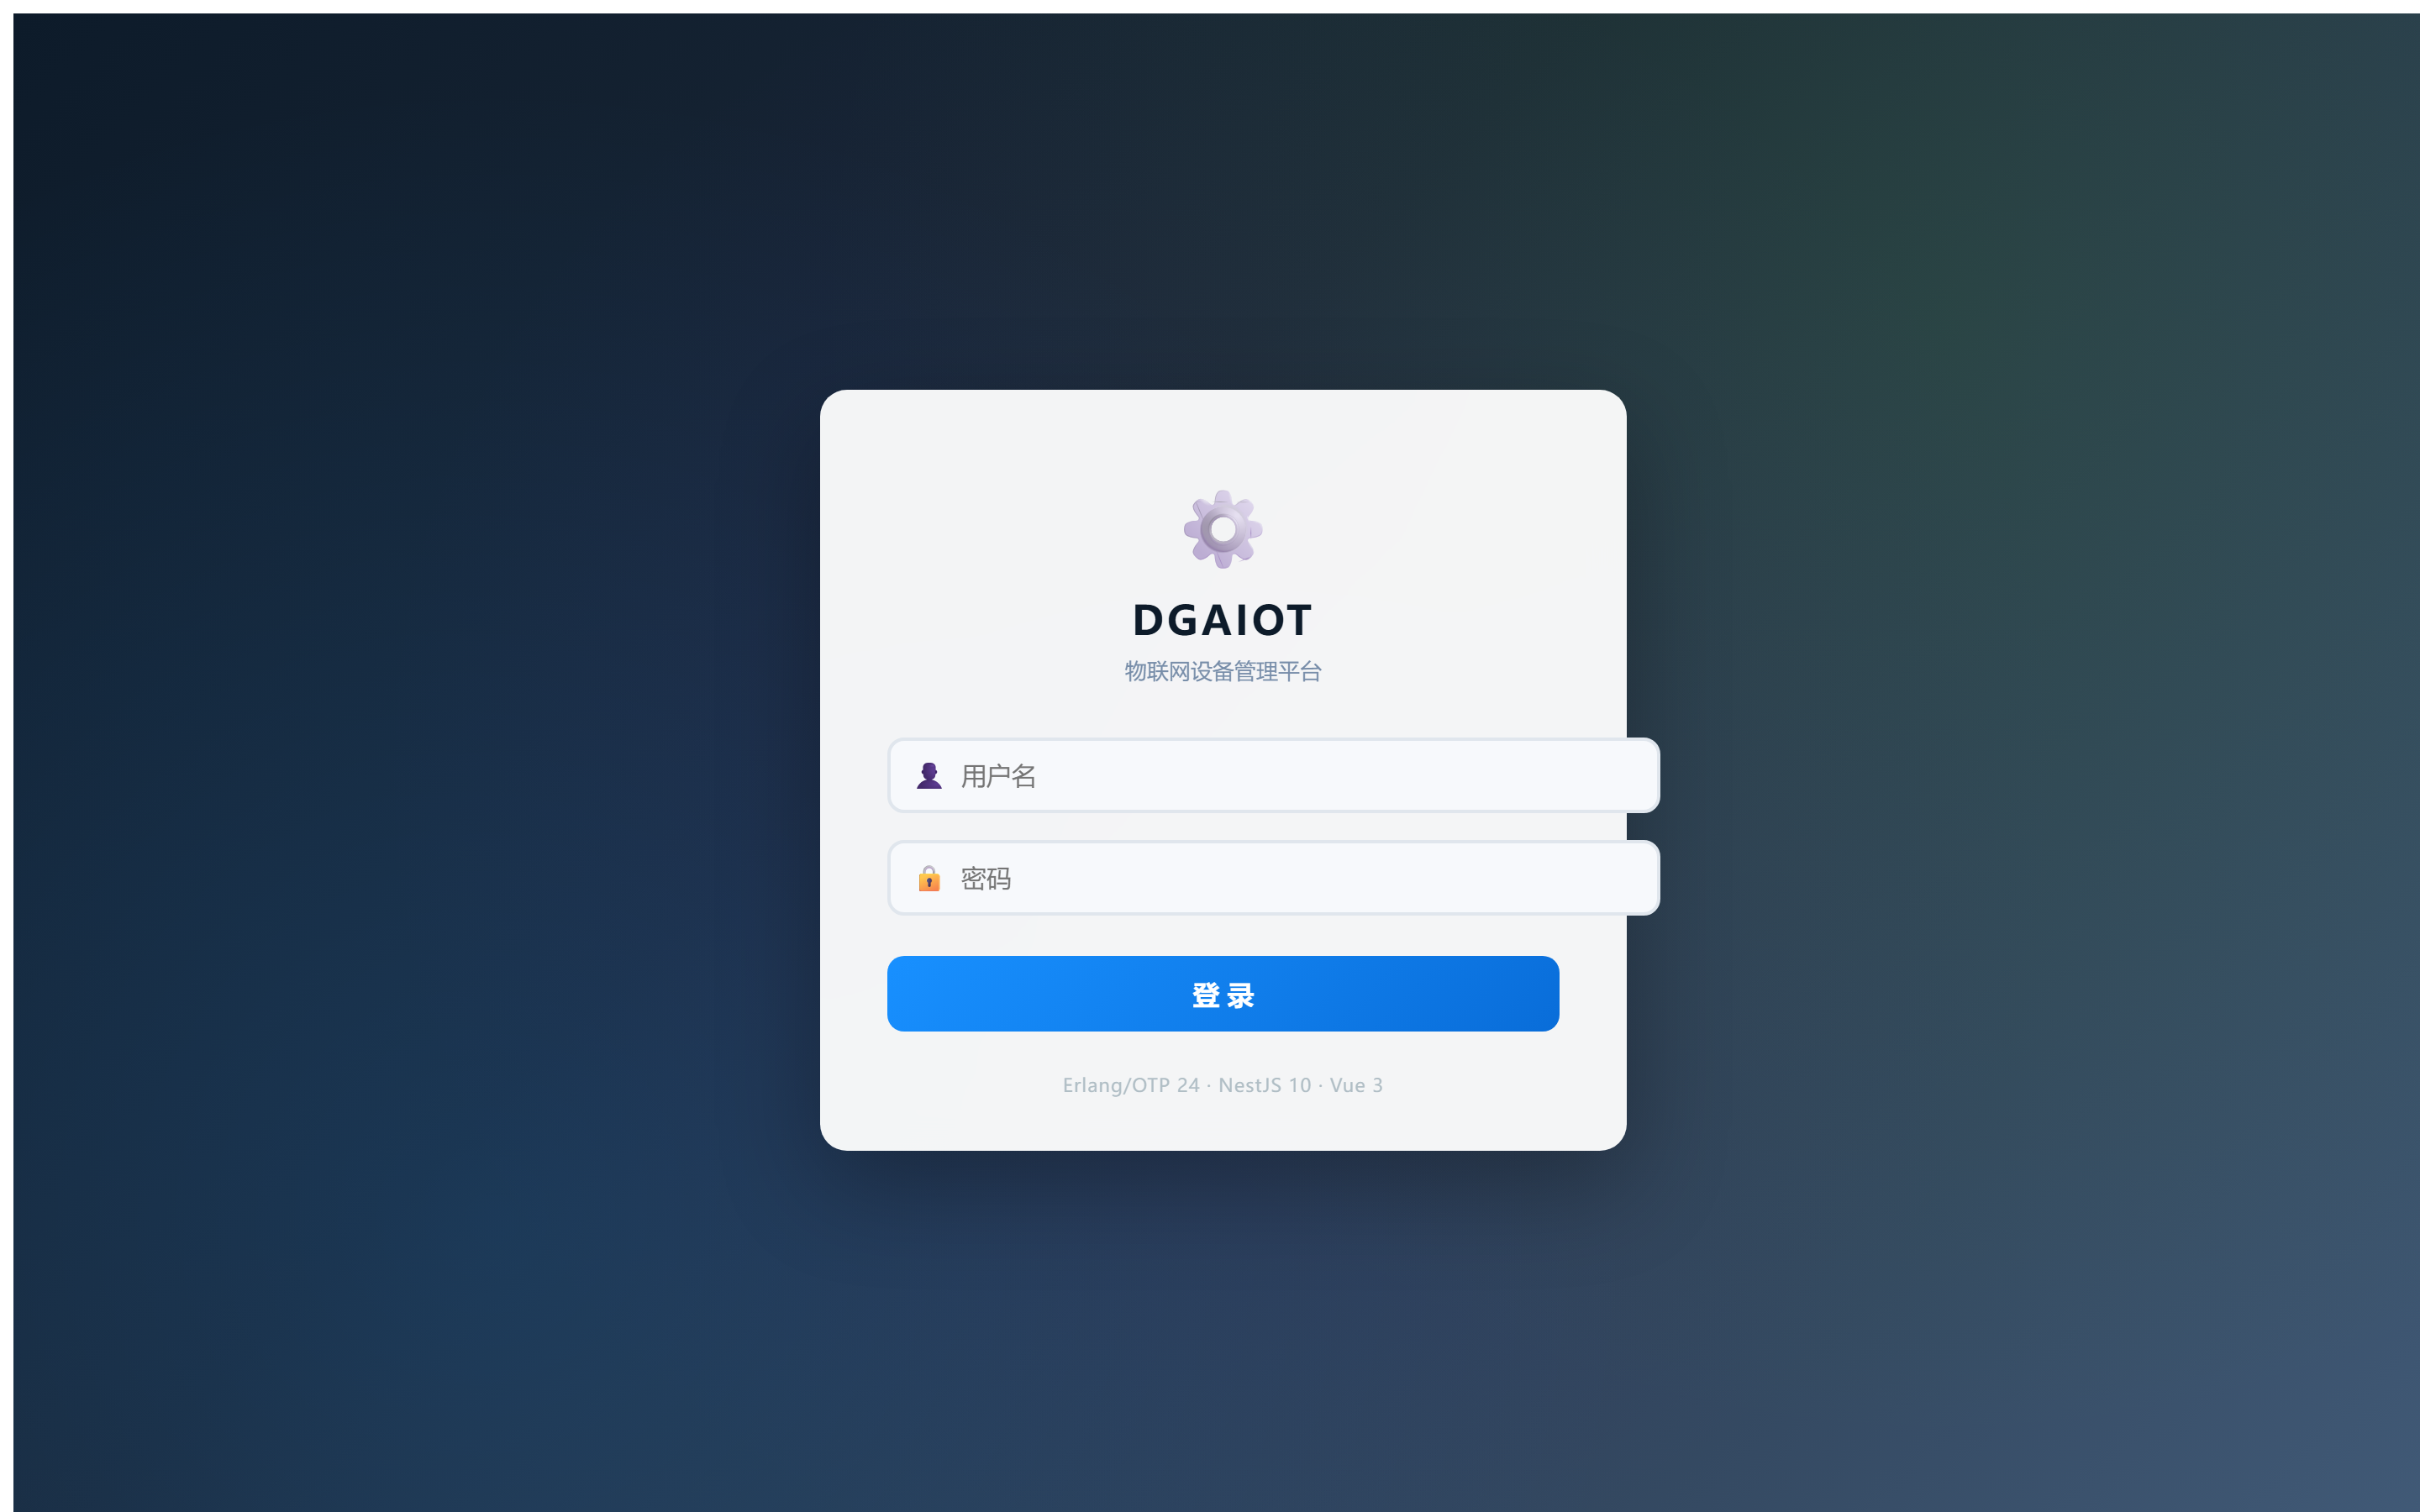
\includegraphics[width=0.92\textwidth]{实际运行-dashboard.png}
\caption{系统实际运行界面——驾驶舱首页}
\end{figure}

\subsection{告警铃铛}

顶部告警铃铛上的红色数字表示当前有多少条未处置告警。点击铃铛弹出告警列表，可直接跳转到告警中心处理。

\section{模块一：驾驶舱}

\begin{figure}[H]\centering
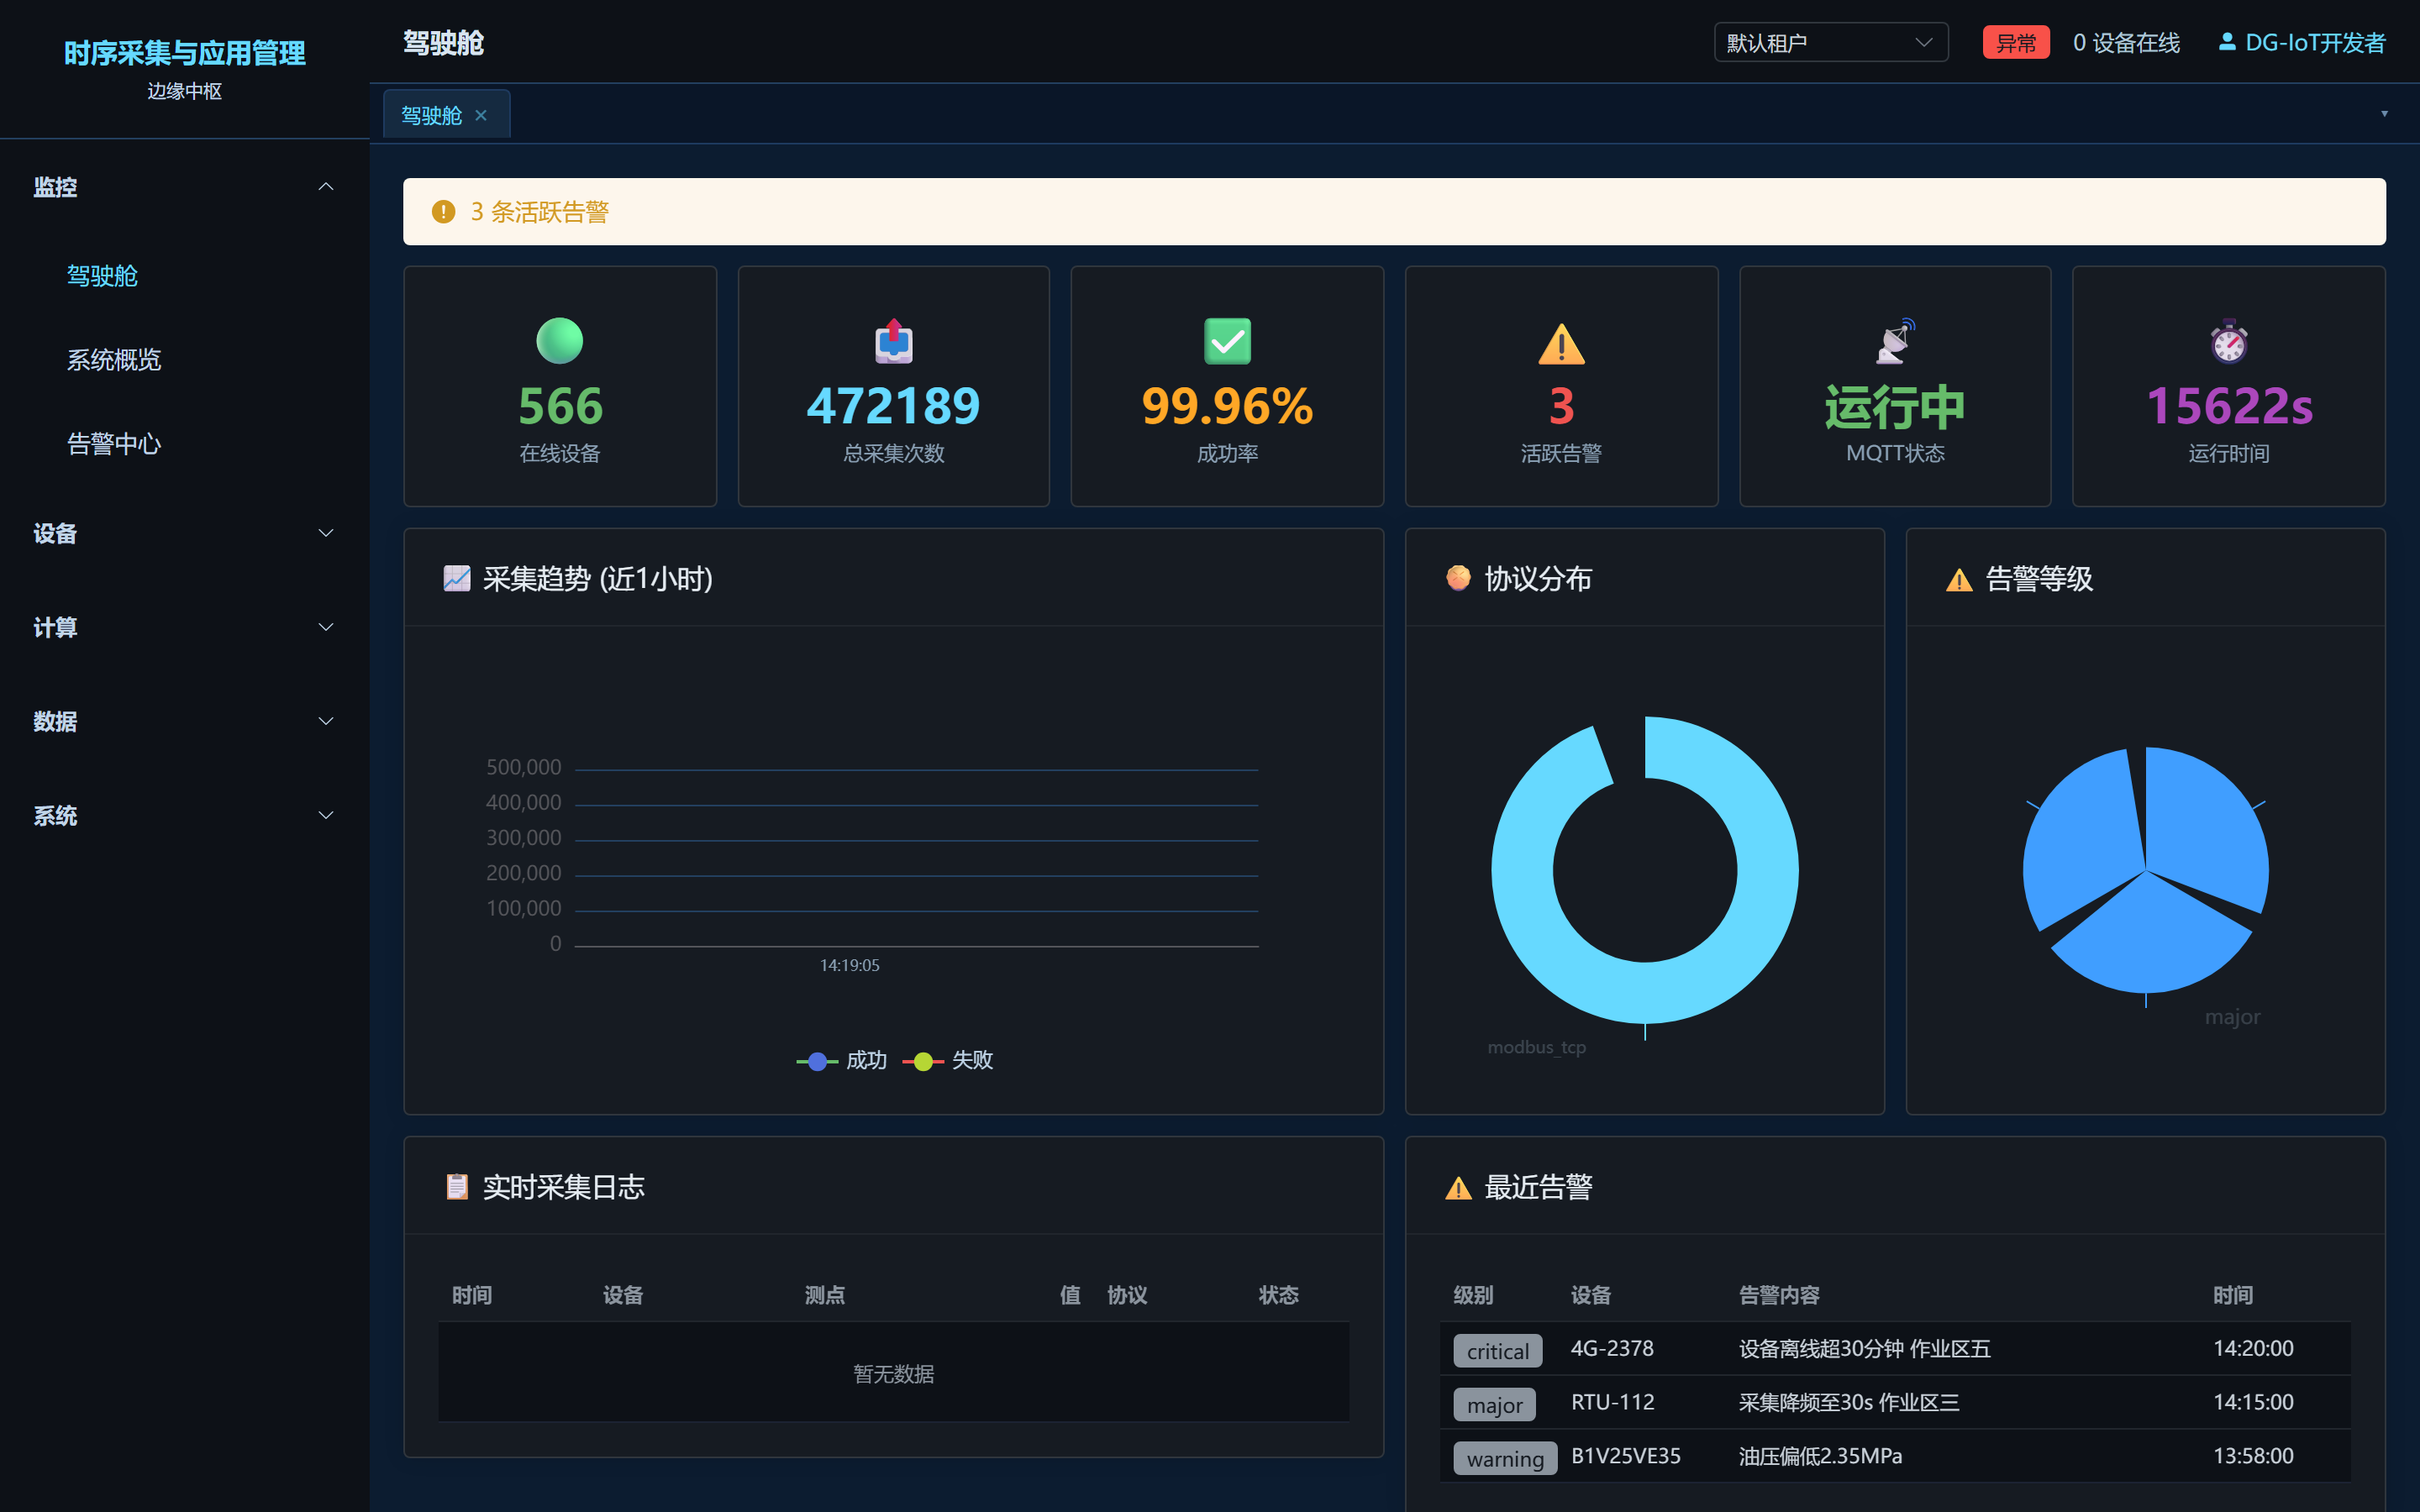
\includegraphics[width=0.92\textwidth]{manual-dashboard.png}
\caption{驾驶舱首页——566设备在线，KPI卡片墙，采集趋势，告警列表}
\end{figure}

\subsection{功能说明}
驾驶舱是系统的首页大屏，用一张图回答"全油田现在是否正常"。

\subsection{界面构成}
\begin{itemize}[leftmargin=*]
  \item \textbf{顶部 KPI 卡片}（自左向右）：链路健康率、采集完整率、设备在线率、今日采集点数。每个卡片显示当前值和较昨日变化
  \item \textbf{中央采集链路拓扑图}：作业区→设备→链路的状态拓扑。绿色=正常、黄色=降频、红色=离线。点击任意节点可下钻查看详情
  \item \textbf{右侧告警滚动列表}：当前未处置告警，严重级别红色高亮，点击跳转告警中心
  \item \textbf{底部采集频率趋势}：近 24 小时全油田采集频率走势
\end{itemize}

\subsection{操作}
\begin{enumerate}[leftmargin=*]
  \item 登录系统后默认进入驾驶舱
  \item 点击任意 KPI 卡片可下钻查看详细数据
  \item 点击拓扑图中的作业区/设备节点可查看该节点详情
  \item 点击告警列表中的条目可跳转到该告警的处置页面
  \item 系统自动刷新（KPI/告警秒级，趋势图 5--30 秒）
\end{enumerate}

\section{模块二：设备管理}

\begin{figure}[H]\centering
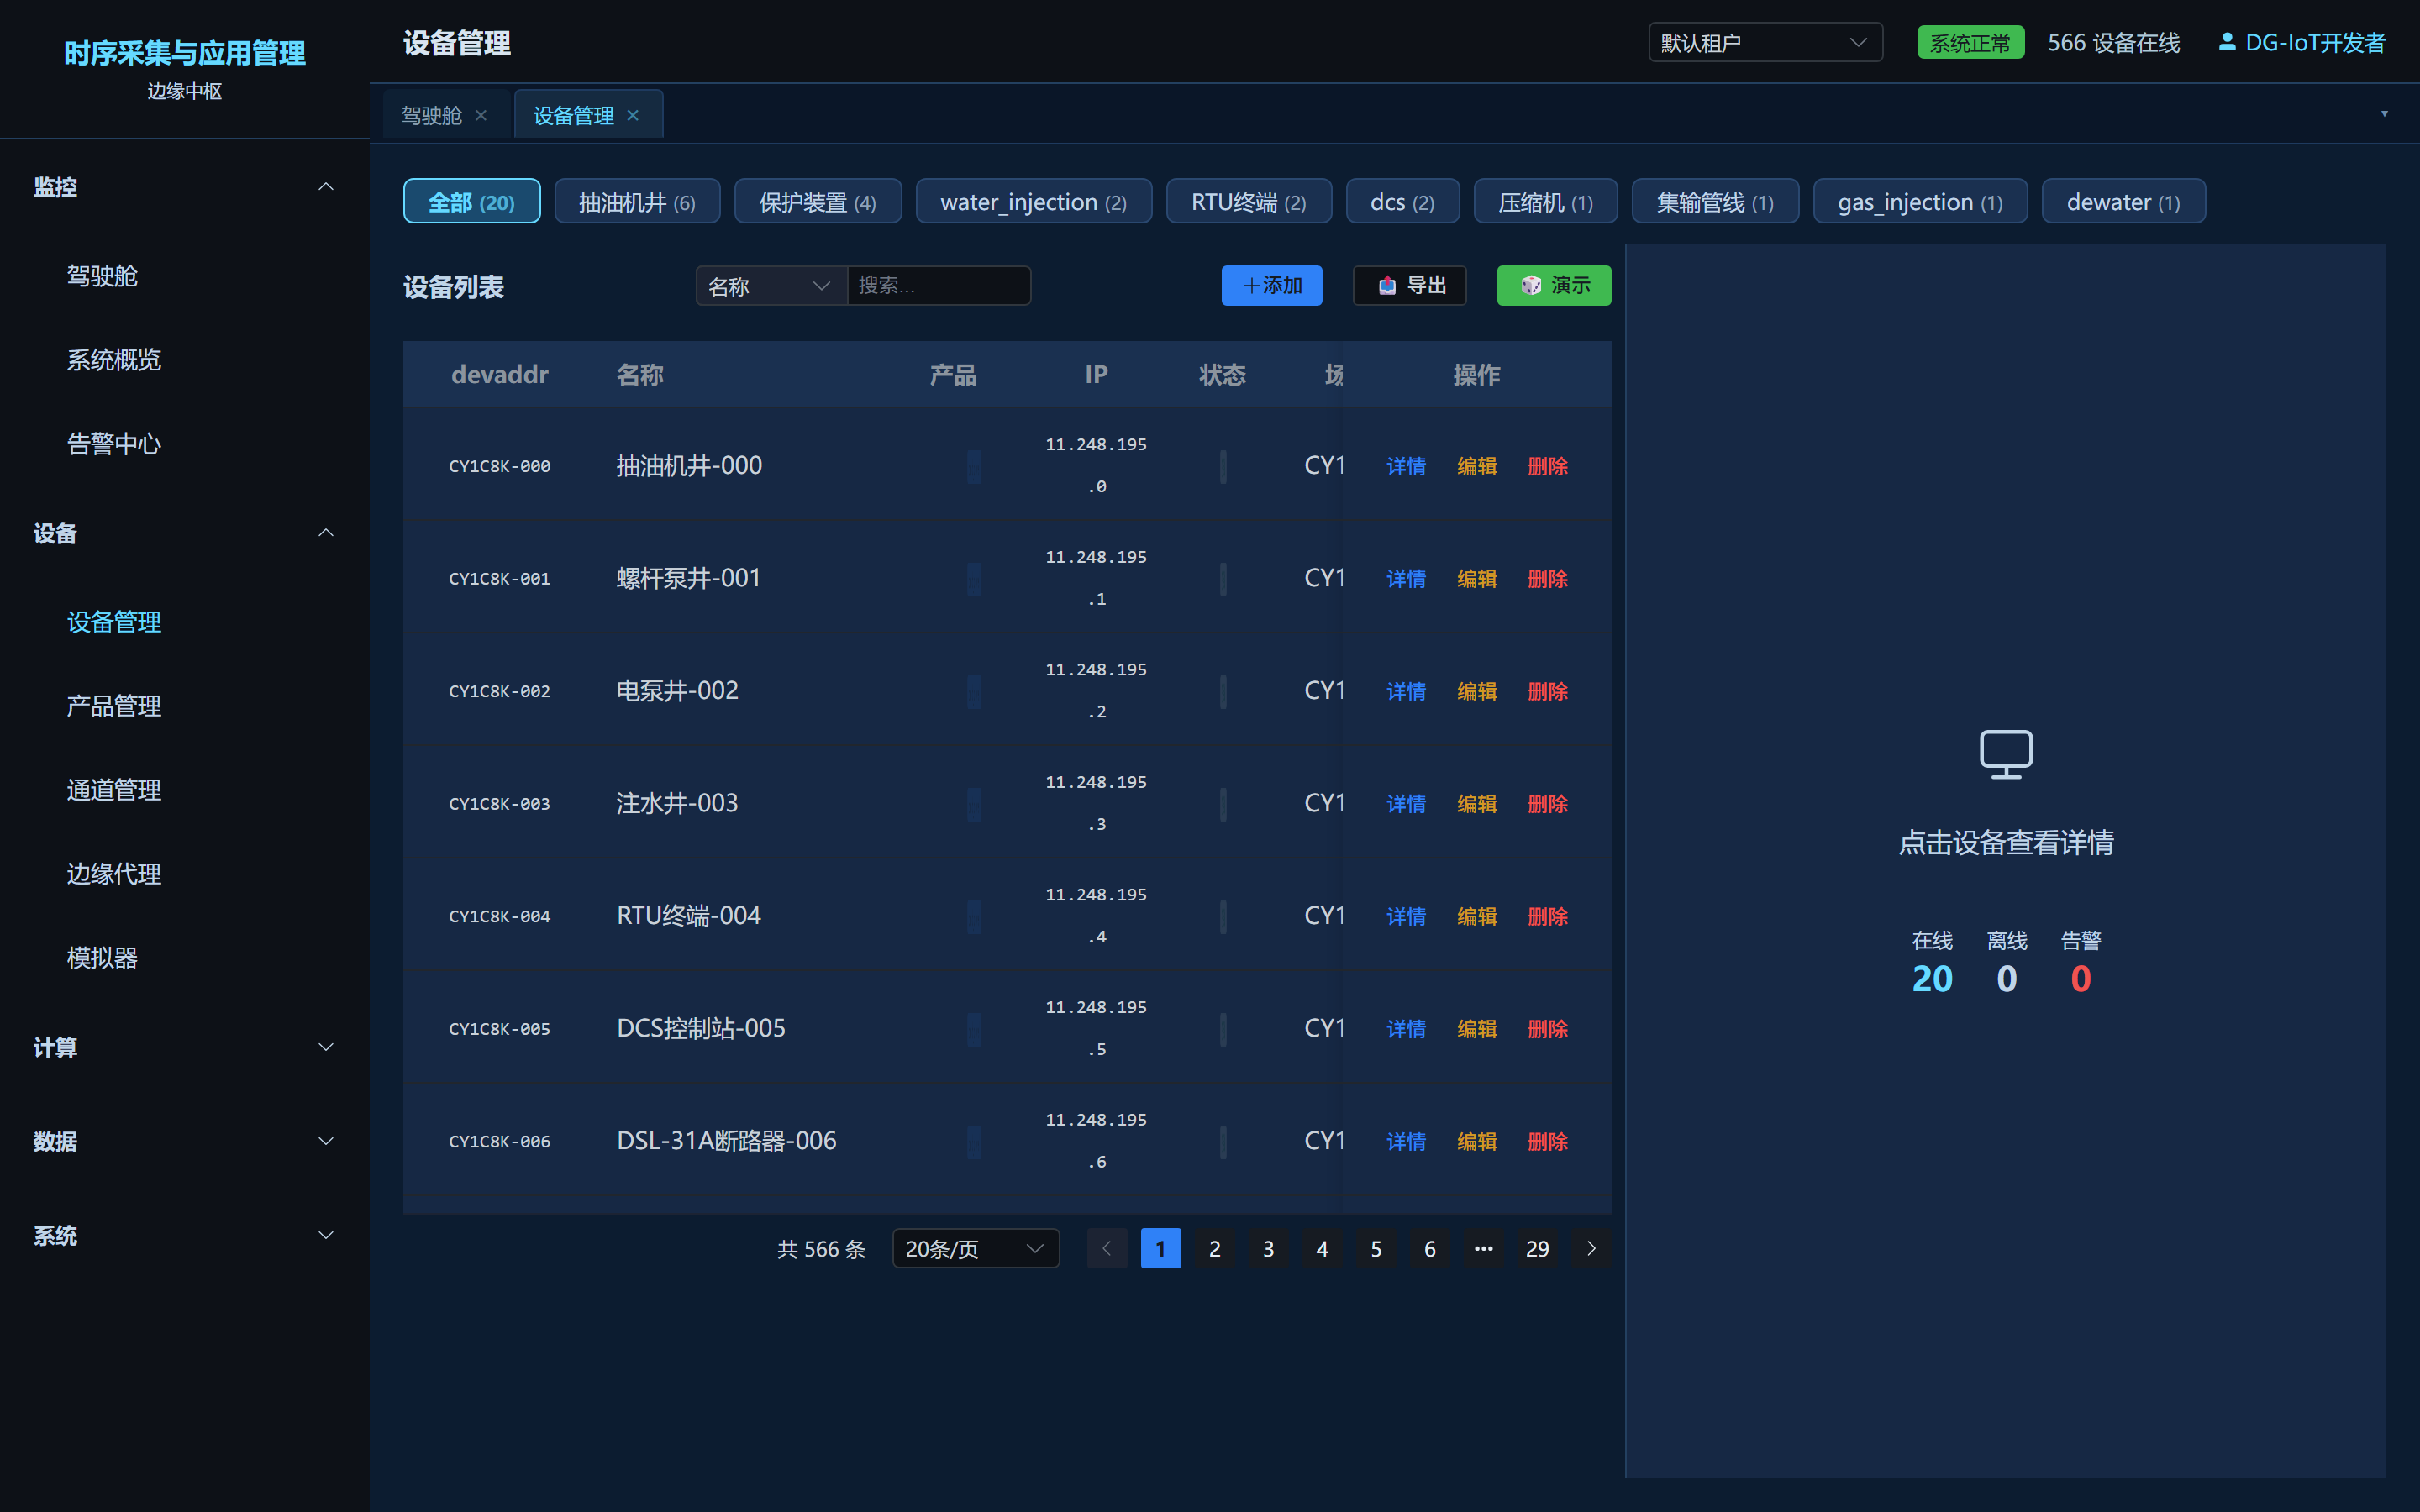
\includegraphics[width=0.92\textwidth]{manual-devices.png}
\caption{设备管理——列表+详情面板，五态生命周期}
\end{figure}

\subsection{功能说明}
管理全油田所有设备的台账信息和运行状态。

\subsection{界面构成}
\begin{itemize}[leftmargin=*]
  \item \textbf{设备列表}：支持按状态筛选（在线/离线/未激活/异常/冻结）、按作业区筛选、按设备类型筛选、关键字搜索
  \item \textbf{设备详情页}（点击设备进入）：六个页签——台账（基本信息）、实时（当前数据）、历史（曲线回放）、告警（关联告警记录）、趋势（趋势分析）、采集日志（采集链路日志）
  \item \textbf{批量操作}：批量导入/导出设备（Excel）、批量修改状态
\end{itemize}

\subsection{操作}
\begin{enumerate}[leftmargin=*]
  \item 在设备列表中使用搜索和筛选找到目标设备
  \item 点击设备名称进入详情页
  \item 在"台账"页签查看和编辑设备基本信息
  \item 在"实时"页签查看设备当前所有测点的实时值
  \item 在"历史"页签拖拽时间轴查看历史曲线
  \item 在"告警"页签查看该设备关联的所有告警记录
\end{enumerate}

\section{模块三：设备接入}

\subsection{功能说明}
监控每台设备的数据采集链路状态，管理采集接入通道。

\subsection{界面构成}
\begin{itemize}[leftmargin=*]
  \item \textbf{终端类型筛选}：静态 IP 终端（有线/固定链路）、动态 IP 终端（4G 移动网关）
  \item \textbf{设备列表}：每台设备的链路状态（正常/降频/离线/告警）、当前采集频率档位、最近数据时间
  \item \textbf{断网补传进度条}：离线设备台数和数据补传进度实时显示
  \item \textbf{网关在线地图}：GIS 视图展示网关分布
\end{itemize}

\subsection{操作}
\begin{enumerate}[leftmargin=*]
  \item 查看链路状态列的颜色判断设备接入是否正常
  \item 对于降频设备，查看降频原因（弱网/低峰/异常加密）
  \item 对于离线设备，查看断网补传区域的进度条确认数据正在补传
  \item 在网关在线地图中查看全油田网关分布和在线状态
\end{enumerate}

\section{模块四：算法管理}

\subsection{功能说明}
管理流水计算算法：查看内置算法、注册定制算法、逐井调优参数。

\subsection{界面构成}
\begin{itemize}[leftmargin=*]
  \item \textbf{内置算法库}：15 种开箱即用的油田算法（工况诊断/预警/统计类），显示每种算法的覆盖率/命中率
  \item \textbf{定制算法注册区}：每作业区 ≥1 种定制算法，支持注册、批量校验
  \item \textbf{逐井调优}：单井参数调整、A/B 版本对比、版本回滚
  \item \textbf{可视化规则编排}：拖拽式配置触发条件与计算动作
\end{itemize}

\subsection{操作}
\begin{enumerate}[leftmargin=*]
  \item 在内置算法库中查看每种算法的命中率，了解算法效果
  \item 点击"注册定制算法"为指定作业区上传和注册定制算法
  \item 使用批量校验功能验证定制算法在大批量历史数据上的表现
  \item 在逐井调优中选择单井，调整算法参数，A/B 对比效果后确认
  \item 在规则编排页面拖拽组件搭建新的计算规则
\end{enumerate}

\section{模块五：告警中心}

\subsection{功能说明}
全油田告警的统一管理和闭环处置。

\subsection{界面构成}
\begin{itemize}[leftmargin=*]
  \item \textbf{告警分级列表}：四级分类（Critical/Error/Warning/Info），严重级别置顶红色标注
  \item \textbf{告警详情}：触发时间、告警等级、关联设备、告警内容、当前状态
  \item \textbf{工单流转}：状态追踪——发现→确认→处置→归档
  \item \textbf{通知记录}：每次通知的方式（声光/短信/平台）、时间、接收人
  \item \textbf{升级链}：超时未确认的告警自动逐级升级通知
\end{itemize}

\subsection{操作}
\begin{enumerate}[leftmargin=*]
  \item 查看告警分级列表，按级别和时间排序处理
  \item 点击告警进入详情，确认告警信息
  \item 确认后分配给处理人员或自行处理
  \item 处理完成后填写处置记录，归档关闭
  \item 超时未处理的告警会自动通过升级链通知上级
\end{enumerate}

\section{模块六：数据服务}

\subsection{功能说明}
查看报表、回放历史数据、获取数据接口。

\subsection{界面构成}
\begin{itemize}[leftmargin=*]
  \item \textbf{报表中心}：日/月/年报表自动生成，支持作业区横向对比
  \item \textbf{历史回放}：时间轴拖拽定位任意时段，曲线回放历史数据
  \item \textbf{健康日报}：设备在线率、采集完整率、采集成功率自动生成
  \item \textbf{REST API 文档}：数据接口说明和在线测试
\end{itemize}

\subsection{操作}
\begin{enumerate}[leftmargin=*]
  \item 在报表中心选择时间范围和作业区，查看或下载报表
  \item 在历史回放中拖拽时间轴到目标时段，查看设备历史曲线
  \item 健康日报每日自动生成，可查看历史日报记录
  \item 在 API 文档中查看可用数据接口和调用示例
\end{enumerate}

\section{模块七：可视化}

\subsection{功能说明}
通过拓扑图、仪表盘、GIS 地图直观展示系统结构和数据。

\subsection{界面构成}
\begin{itemize}[leftmargin=*]
  \item \textbf{采集链路拓扑图}：作业区→设备→链路逐级展开，状态着色
  \item \textbf{拖拽式仪表盘}：自由拖拽图表、指标卡、趋势图组件搭建个性化仪表盘
  \item \textbf{GIS 地图}：油田→作业区→站库层级下钻，设备点位标注
\end{itemize}

\subsection{操作}
\begin{enumerate}[leftmargin=*]
  \item 在拓扑图中点击任意节点下钻查看详情
  \item 在仪表盘编辑模式中拖拽图表组件到画布
  \item 配置每个图表的数据源和显示参数
  \item 保存模板，下次直接加载
  \item 在 GIS 地图上点击设备图标查看设备详情
\end{enumerate}

\section{模块八：自动化}

\subsection{功能说明}
配置自动联动规则和场景编排，减少人工干预。

\subsection{界面构成}
\begin{itemize}[leftmargin=*]
  \item \textbf{规则引擎}：IF-THEN 规则——采集触发 → 条件判定 → 动作执行
  \item \textbf{场景编排}：批量设备配置下发、定时巡检任务、断网自动补传触发
  \item \textbf{设备影子}：显示上报值 vs 期望值，支持远程配置下发
\end{itemize}

\subsection{操作}
\begin{enumerate}[leftmargin=*]
  \item 在规则引擎中创建新规则：选择触发条件→设置判定逻辑→配置执行动作
  \item 在场景编排中选择模板（如"批量调频"、"定时巡检"），配置参数后启用
  \item 在设备影子中查看设备当前状态，必要时下发配置变更
\end{enumerate}

\section{模块九：系统管理}

\subsection{功能说明}
管理用户权限、审计日志、安全配置。

\subsection{界面构成}
\begin{itemize}[leftmargin=*]
  \item \textbf{用户管理}：创建/编辑/禁用用户，分配角色
  \item \textbf{角色管理}：三种角色——领导视图（只看驾驶舱）、调度视图（驾驶舱+告警+报表）、运维视图（全部功能）
  \item \textbf{审计日志}：操作全留痕——谁、什么时间、做了什么操作、IP 地址
  \item \textbf{安全配置}：国密算法开关、密码策略、会话超时设置
\end{itemize}

\subsection{操作}
\begin{enumerate}[leftmargin=*]
  \item 在用户管理中创建新用户，选择对应角色
  \item 在角色管理中查看和调整角色的界面访问权限
  \item 在审计日志中按时间、用户、操作类型搜索
  \item 在安全配置中查看和调整安全策略
\end{enumerate}

\section{常见问题}

\textbf{Q: 驾驶舱上的数字是实时的吗？}\\
A: KPI 和告警是秒级刷新（WebSocket 推送），趋势曲线每 5--30 秒刷新一次。

\textbf{Q: 设备离线了数据会丢吗？}\\
A: 不会。边缘代理有本地缓存，网络恢复后自动按时间顺序补传，去重不丢。

\textbf{Q: A11 系统的数据还能用吗？}\\
A: 能。A11 系统完全保留不动，本系统在 A11 旁边并行一条新通道，不影响 A11 任何业务。

\textbf{Q: 新作业区加入需要重新部署吗？}\\
A: 不需要。边缘代理按作业区独立部署，新作业区部署一台 IO 服务器的代理即可接入。

\textbf{Q: 怎么知道哪个作业区有异常？}\\
A: 驾驶舱中间拓扑图会标红异常设备和作业区，右侧告警列表按严重程度排列，点击即可下钻。

\vspace{1em}\noindent\hrulefill
\begin{center}\small
编制单位：迪格(杭州)物联科技有限公司 \quad 2026-08
\end{center}

\end{document}
